\documentclass[10pt,a4paper]{article}

% --- Page Geometry & Margins ---
\usepackage[top=0.6in, bottom=0.6in, left=0.7in, right=0.7in]{geometry}

% --- Typography & Encodings ---
\usepackage[utf8]{inputenc}
\usepackage[T1]{fontenc}
\usepackage{lmodern}
\usepackage{microtype}
\usepackage{amsmath, amssymb}
\usepackage{multicol}

% --- Graphics, Colors & Tables ---
\usepackage{graphicx}
\usepackage[table,xcdraw]{xcolor}
\usepackage{booktabs}
\usepackage{tabularx}
\usepackage{array}
\usepackage{enumitem}

% --- Framing & Boxes ---
\usepackage{tcolorbox}
\tcbuselibrary{skins,breakable}

% --- TikZ & Diagram Libraries ---
\usepackage{tikz}
\usetikzlibrary{shapes.geometric, arrows.meta, positioning, calc, fit, backgrounds, decorations.pathreplacing, shadows}

% --- Headers & Footers ---
\usepackage{fancyhdr}
\pagestyle{fancy}
\fancyhf{}
\renewcommand{\headrulewidth}{0.4pt}
\renewcommand{\footrulewidth}{0.4pt}
\fancyhead[L]{\small\textbf{CVIS} --- Connected Vehicle Intelligence System}
\fancyhead[R]{\small\textbf{Faculty Architectural \& CCNS Reference Guide}}
\fancyfoot[L]{\footnotesize Computer Communication \& Network Security (CCNS) Course Reference}
\fancyfoot[C]{\textbf{\thepage\ of 5}}
\fancyfoot[R]{\footnotesize SRM Institute of Science and Technology}

% --- Hyperlinks ---
\usepackage{hyperref}
\hypersetup{
    colorlinks=true,
    linkcolor=cvisblue,
    citecolor=cvisblue,
    urlcolor=cvisblue
}

% --- Color Palette (Automotive Tech Theme) ---
\definecolor{cvisblue}{RGB}{14, 116, 144}      % Deep Cyan/Blue
\definecolor{cvisnavy}{RGB}{15, 23, 42}        % Dark Slate Header
\definecolor{cviscyan}{RGB}{6, 182, 212}       % Bright Cyan
\definecolor{cvisgreen}{RGB}{16, 185, 129}     % Emerald Green
\definecolor{cvisred}{RGB}{239, 68, 68}        % Alert Red
\definecolor{cvisorange}{RGB}{245, 158, 11}    % Amber Warning
\definecolor{cvispurple}{RGB}{139, 92, 246}    % Accent Purple
\definecolor{cvisdark}{RGB}{30, 41, 59}        % Slate 800
\definecolor{cvislight}{RGB}{248, 250, 252}    % Slate 50
\definecolor{cvisborder}{RGB}{203, 213, 225}   % Slate 300

% --- TikZ Global Styles ---
\tikzset{
    baseblock/.style={
        rectangle, rounded corners=3pt, draw=cvisdark, line width=0.8pt,
        align=center, font=\footnotesize, fill=white, drop shadow={opacity=0.15, shadow xshift=1pt, shadow yshift=-1pt}
    },
    vehicleblock/.style={
        baseblock, fill=blue!5, draw=cvisblue, line width=1pt
    },
    gatewayblock/.style={
        baseblock, fill=orange!5, draw=cvisorange, line width=1pt
    },
    backendblock/.style={
        baseblock, fill=green!5, draw=cvisgreen, line width=1pt
    },
    aiblock/.style={
        baseblock, fill=purple!5, draw=cvispurple, line width=1pt
    },
    uiblock/.style={
        baseblock, fill=cyan!5, draw=cviscyan, line width=1pt
    },
    securityblock/.style={
        baseblock, fill=red!5, draw=cvisred, line width=1pt
    },
    flowarrow/.style={
        -{Stealth[length=5pt, width=4pt]}, line width=1.1pt, draw=cvisdark
    },
    bidirarrow/.style={
        {Stealth[length=4pt, width=3pt]}-{Stealth[length=4pt, width=3pt]}, line width=1pt, draw=cvisdark
    },
    dasharrow/.style={
        -{Stealth[length=4pt, width=3pt]}, line width=0.9pt, dashed, draw=cvisblue
    },
    groupbox/.style={
        draw=cvisdark!60, line width=0.8pt, dashed, rounded corners=6pt, fill=black!2, inner sep=6pt
    }
}

\begin{document}

% ==============================================================================
% PAGE 1: ARCHITECTURAL DIAGRAM OF THE PROJECT
% ==============================================================================
\noindent
\begin{tcolorbox}[colback=cvisnavy, colframe=cvisnavy, arc=4pt, boxrule=0pt, coltext=white, left=8pt, right=8pt, top=6pt, bottom=6pt]
    \begin{minipage}{0.72\textwidth}
        {\Large \textbf{CONNECTED VEHICLE INTELLIGENCE SYSTEM (CVIS)}}\\[2pt]
        {\small \textbf{Project Identity \& System Architecture Reference Guide}}\\[2pt]
        {\footnotesize \textbf{Course:} 21ECC402P --- Computer Communication and Network Security (CCNS) $|$ \textbf{Author:} Justin Jacob Saju}
    \end{minipage}%
    \begin{minipage}{0.28\textwidth}
        \raggedleft
        \tcbox[colback=cviscyan, colframe=white, boxrule=0.5pt, arc=3pt, top=2pt, bottom=2pt, left=4pt, right=4pt]{
            \textcolor{cvisnavy}{\textbf{\footnotesize PAGE 1: SYSTEM ARCHITECTURE}}
        }\par\vspace{2pt}
        {\scriptsize \textbf{Evaluation Target:} Academic / Faculty Defense}
    \end{minipage}
\end{tcolorbox}

\vspace{-6pt}
\begin{tcolorbox}[colback=cvislight, colframe=cvisblue, boxrule=0.8pt, arc=3pt, left=6pt, right=6pt, top=4pt, bottom=4pt]
    \textbf{\footnotesize Core Academic Thesis:} Vehicles must \textbf{not} run heavy neural models directly on resource/thermally-constrained in-vehicle ECUs. The vehicle is designed as a \textbf{thin, hardened, cryptographically secure networked client}. The compute-intensive AI lives centrally in the cloud/edge data center. This project implements and demonstrates the \textbf{secure, fault-tolerant communication and network security layer} that makes this architecture viable, verifiable, and economically scalable.
\end{tcolorbox}

\vspace{-4pt}
\begin{center}
\resizebox{0.99\textwidth}{!}{
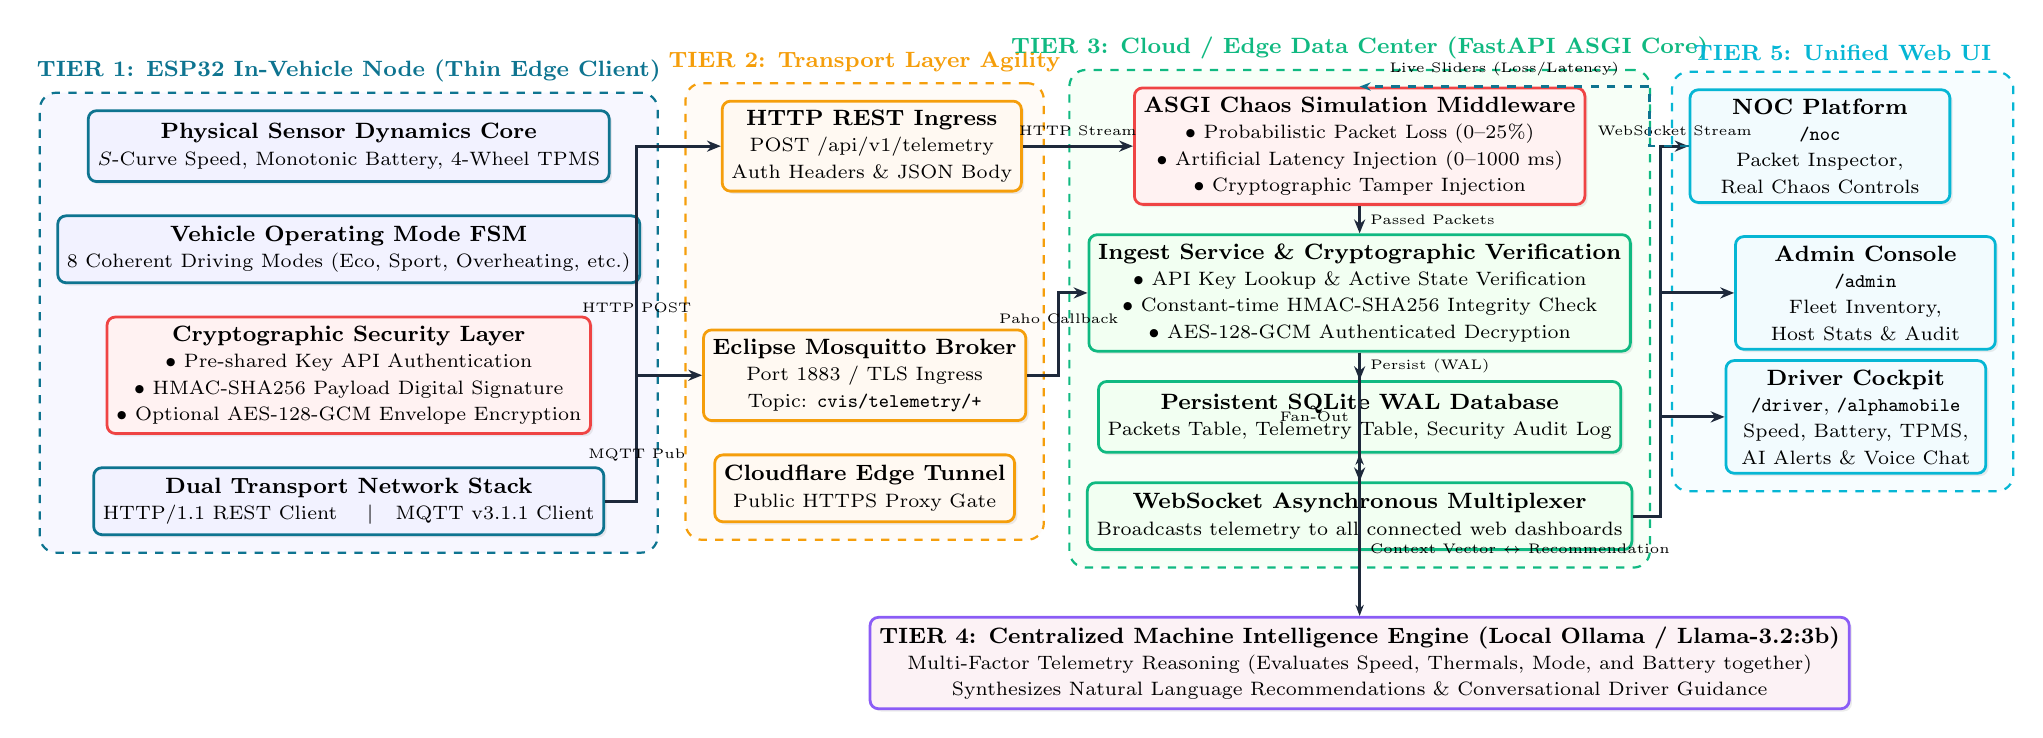
\begin{tikzpicture}[node distance=1.1cm]

    % --- LAYER 1: VEHICLE NODE LAYER (EDGE CLIENT) ---
    \node[vehicleblock, minimum width=4.3cm, minimum height=0.9cm] (sensors) {
        \textbf{Physical Sensor Dynamics Core}\\
        \scriptsize $S$-Curve Speed, Monotonic Battery, 4-Wheel TPMS
    };

    \node[vehicleblock, below=0.4cm of sensors, minimum width=4.3cm, minimum height=0.85cm] (fsm) {
        \textbf{Vehicle Operating Mode FSM}\\
        \scriptsize 8 Coherent Driving Modes (Eco, Sport, Overheating, etc.)
    };

    \node[securityblock, below=0.4cm of fsm, minimum width=4.3cm, minimum height=0.95cm] (firmware_sec) {
        \textbf{Cryptographic Security Layer}\\
        \scriptsize $\bullet$ Pre-shared Key API Authentication\\
        \scriptsize $\bullet$ HMAC-SHA256 Payload Digital Signature\\
        \scriptsize $\bullet$ Optional AES-128-GCM Envelope Encryption
    };

    \node[vehicleblock, below=0.4cm of firmware_sec, minimum width=4.3cm, minimum height=0.85cm] (transports) {
        \textbf{Dual Transport Network Stack}\\
        \scriptsize HTTP/1.1 REST Client \quad$|$\quad MQTT v3.1.1 Client
    };

    \begin{scope}[on background layer]
        \node[groupbox, fit=(sensors) (fsm) (firmware_sec) (transports), fill=blue!3, draw=cvisblue, label={[cvisblue, font=\bfseries\footnotesize]north:\textbf{TIER 1: ESP32 In-Vehicle Node (Thin Edge Client)}}] (box_vehicle) {};
    \end{scope}

    % --- LAYER 2: TRANSPORT & INGRESS LAYER ---
    \node[gatewayblock, right=1.4cm of sensors, minimum width=3.4cm, minimum height=1.1cm] (http_link) {
        \textbf{HTTP REST Ingress}\\
        \scriptsize POST /api/v1/telemetry\\
        \scriptsize Auth Headers \& JSON Body
    };

    \node[gatewayblock, right=1.4cm of firmware_sec, minimum width=3.4cm, minimum height=1.1cm] (mqtt_broker) {
        \textbf{Eclipse Mosquitto Broker}\\
        \scriptsize Port 1883 / TLS Ingress\\
        \scriptsize Topic: \texttt{cvis/telemetry/+}
    };

    \node[gatewayblock, below=0.4cm of mqtt_broker, minimum width=3.4cm, minimum height=0.85cm] (tunnel) {
        \textbf{Cloudflare Edge Tunnel}\\
        \scriptsize Public HTTPS Proxy Gate
    };

    \begin{scope}[on background layer]
        \node[groupbox, fit=(http_link) (mqtt_broker) (tunnel), fill=orange!3, draw=cvisorange, label={[cvisorange, font=\bfseries\footnotesize]north:\textbf{TIER 2: Transport Layer Agility}}] (box_transport) {};
    \end{scope}

    % --- LAYER 3: CLOUD / DATA CENTER BACKEND ---
    \node[securityblock, right=1.4cm of http_link, minimum width=4.8cm, minimum height=1.15cm] (chaos) {
        \textbf{ASGI Chaos Simulation Middleware}\\
        \scriptsize $\bullet$ Probabilistic Packet Loss (0--25\%)\\
        \scriptsize $\bullet$ Artificial Latency Injection (0--1000 ms)\\
        \scriptsize $\bullet$ Cryptographic Tamper Injection
    };

    \node[backendblock, below=0.35cm of chaos, minimum width=4.8cm, minimum height=1.15cm] (ingest_sec) {
        \textbf{Ingest Service \& Cryptographic Verification}\\
        \scriptsize $\bullet$ API Key Lookup \& Active State Verification\\
        \scriptsize $\bullet$ Constant-time HMAC-SHA256 Integrity Check\\
        \scriptsize $\bullet$ AES-128-GCM Authenticated Decryption
    };

    \node[backendblock, below=0.35cm of ingest_sec, minimum width=4.8cm, minimum height=0.9cm] (storage) {
        \textbf{Persistent SQLite WAL Database}\\
        \scriptsize Packets Table, Telemetry Table, Security Audit Log
    };

    \node[backendblock, below=0.35cm of storage, minimum width=4.8cm, minimum height=0.85cm] (ws_engine) {
        \textbf{WebSocket Asynchronous Multiplexer}\\
        \scriptsize Broadcasts telemetry to all connected web dashboards
    };

    \begin{scope}[on background layer]
        \node[groupbox, fit=(chaos) (ingest_sec) (storage) (ws_engine), fill=green!3, draw=cvisgreen, label={[cvisgreen, font=\bfseries\footnotesize]north:\textbf{TIER 3: Cloud / Edge Data Center (FastAPI ASGI Core)}}] (box_backend) {};
    \end{scope}

    % --- LAYER 4: INTELLIGENCE & PRESENTATION ---
    \node[aiblock, below=0.6cm of box_backend, minimum width=7.2cm, minimum height=1.05cm] (ai_engine) {
        \textbf{TIER 4: Centralized Machine Intelligence Engine (Local Ollama / Llama-3.2:3b)}\\
        \scriptsize Multi-Factor Telemetry Reasoning (Evaluates Speed, Thermals, Mode, and Battery together)\\
        \scriptsize Synthesizes Natural Language Recommendations \& Conversational Driver Guidance
    };

    \node[uiblock, right=1.3cm of chaos, minimum width=3.3cm, minimum height=1.15cm] (noc_ui) {
        \textbf{NOC Platform}\\
        \scriptsize \texttt{/noc}\\
        \scriptsize Packet Inspector,\\
        \scriptsize Real Chaos Controls
    };

    \node[uiblock, right=1.3cm of ingest_sec, minimum width=3.3cm, minimum height=1.15cm] (admin_ui) {
        \textbf{Admin Console}\\
        \scriptsize \texttt{/admin}\\
        \scriptsize Fleet Inventory,\\
        \scriptsize Host Stats \& Audit
    };

    \node[uiblock, right=1.3cm of storage, minimum width=3.3cm, minimum height=1.15cm] (driver_ui) {
        \textbf{Driver Cockpit}\\
        \scriptsize \texttt{/driver}, \texttt{/alphamobile}\\
        \scriptsize Speed, Battery, TPMS,\\
        \scriptsize AI Alerts \& Voice Chat
    };

    \begin{scope}[on background layer]
        \node[groupbox, fit=(noc_ui) (admin_ui) (driver_ui), fill=cyan!3, draw=cviscyan, label={[cviscyan, font=\bfseries\footnotesize]north:\textbf{TIER 5: Unified Web UI}}] (box_ui) {};
    \end{scope}

    % --- CONNECTING FLOW ARROWS ---
    \draw[flowarrow] (transports.east) -- ++(0.4,0) |- (http_link.west) node[near start, above, font=\tiny] {HTTP POST};
    \draw[flowarrow] (transports.east) -- ++(0.4,0) |- (mqtt_broker.west) node[near start, below, font=\tiny] {MQTT Pub};
    
    \draw[flowarrow] (http_link.east) -- (chaos.west) node[midway, above, font=\tiny] {HTTP Stream};
    \draw[flowarrow] (mqtt_broker.east) -- ++(0.4,0) |- (ingest_sec.west) node[near start, above, font=\tiny] {Paho Callback};

    \draw[flowarrow] (chaos.south) -- (ingest_sec.north) node[midway, right, font=\tiny] {Passed Packets};
    \draw[flowarrow] (ingest_sec.south) -- (storage.north) node[midway, right, font=\tiny] {Persist (WAL)};
    \draw[flowarrow] (ingest_sec.south) -- ++(0,0) -| (ws_engine.north) node[near end, left, font=\tiny] {Fan-Out};

    \draw[bidirarrow] (storage.south) -- ++(0,-0.35) -| (ai_engine.north) node[near end, right, font=\tiny] {Context Vector $\leftrightarrow$ Recommendation};

    \draw[flowarrow] (ws_engine.east) -- ++(0.35,0) |- (noc_ui.west) node[near end, above, font=\tiny] {WebSocket Stream};
    \draw[flowarrow] (ws_engine.east) -- ++(0.35,0) |- (admin_ui.west);
    \draw[flowarrow] (ws_engine.east) -- ++(0.35,0) |- (driver_ui.west);

    \draw[dasharrow] (noc_ui.west) -- ++(-0.5,0) |- (chaos.north) node[near end, above, font=\tiny] {Live Sliders (Loss/Latency)};

\end{tikzpicture}
}
\end{center}

\vspace{-8pt}
\begin{table}[h!]
\centering
\scriptsize
\begin{tabularx}{\textwidth}{p{2.6cm}p{3.8cm}p{4.2cm}p{4.8cm}}
\toprule
\textbf{Architectural Tier} & \textbf{Component Implementation} & \textbf{Primary Engineering Responsibility} & \textbf{Demonstrated CCNS Syllabus Concept} \\
\midrule
\textbf{Tier 1: Vehicle Node} & ESP32 / C++ Firmware / FreeRTOS & Sensor simulation, 8-mode FSM, HMAC signing & Lightweight client security, message integrity \\
\textbf{Tier 2: Transport Layer} & HTTP REST + Eclipse Mosquitto & Dual-protocol transmission, runtime agility & OSI Model, Protocol Interoperability, Transport comparison \\
\textbf{Tier 3: Cloud / Backend} & FastAPI, SQLite WAL, ASGI & Middleware chaos injection, crypto verification & Access Control, HMAC validation, DOS/Loss resilience \\
\textbf{Tier 4: Intelligence} & Ollama Local SLM (Llama-3.2:3b) & Multi-sensor semantic telemetry analysis & Cloud AI application layer riding securely on network \\
\textbf{Tier 5: Presentation} & Unified Next.js 16 (React, Tailwind) & Role-based Driver, NOC, and Admin monitoring & Network Operations Center (NOC), auditability, HUD \\
\bottomrule
\end{tabularx}
\end{table}

\clearpage
% ==============================================================================
% PAGE 2: DIAGRAMMATIC REPRESENTATION OF THE PROJECT WORKING
% ==============================================================================
\noindent
\begin{tcolorbox}[colback=cvisnavy, colframe=cvisnavy, arc=4pt, boxrule=0pt, coltext=white, left=8pt, right=8pt, top=6pt, bottom=6pt]
    \begin{minipage}{0.72\textwidth}
        {\Large \textbf{PROJECT WORKING \& RUNTIME DATA FLOW LIFECYCLE}}\\[2pt]
        {\small \textbf{Step-by-Step Operational Lifecycle: Sensor Acquisition to Decision Fan-Out}}\\[2pt]
        {\footnotesize \textbf{Course:} 21ECC402P --- Computer Communication and Network Security (CCNS)}
    \end{minipage}%
    \begin{minipage}{0.28\textwidth}
        \raggedleft
        \tcbox[colback=cvisgreen, colframe=white, boxrule=0.5pt, arc=3pt, top=2pt, bottom=2pt, left=4pt, right=4pt]{
            \textcolor{white}{\textbf{\footnotesize PAGE 2: RUNTIME FLOW}}
        }\par\vspace{2pt}
        {\scriptsize \textbf{Stage:} Ingestion \& Verification Pipeline}
    \end{minipage}
\end{tcolorbox}

\vspace{-6pt}
\begin{tcolorbox}[colback=cvislight, colframe=cvisgreen, boxrule=0.8pt, arc=3pt, left=6pt, right=6pt, top=4pt, bottom=4pt]
    \textbf{\footnotesize Operational Overview:} Telemetry follows a strict, verifiable 8-stage pipeline. The vehicle samples dynamic physics parameters, constructs an authenticated cryptographic frame, and dispatches it over the active network protocol. The cloud middleware applies software-defined network chaos (testing real-world degradation), validates identity and cryptographic integrity, persists the raw wire payload into write-ahead logs, invokes multi-factor artificial intelligence, and fans out updates to live operations dashboards in sub-5ms latency.
\end{tcolorbox}

\vspace{-4pt}
\begin{center}
\resizebox{0.99\textwidth}{!}{
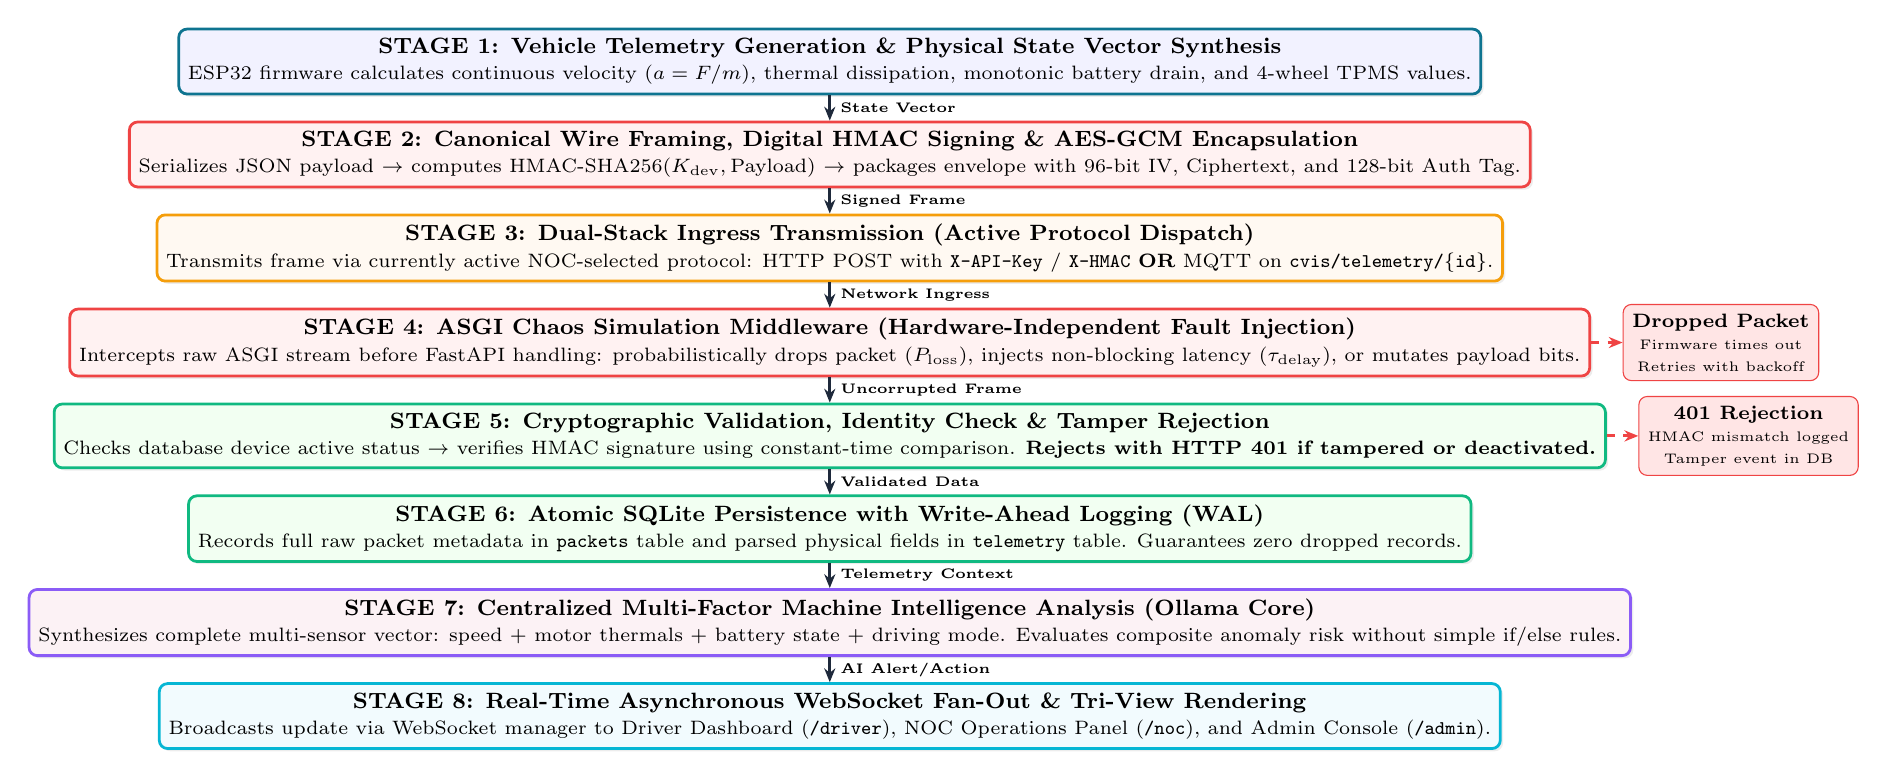
\begin{tikzpicture}[node distance=0.9cm]

    % --- FLOW NODES: STEP 1 TO STEP 8 ---
    \node[vehicleblock, minimum width=12cm, minimum height=0.75cm] (s1) {
        \textbf{STAGE 1: Vehicle Telemetry Generation \& Physical State Vector Synthesis}\\
        \scriptsize ESP32 firmware calculates continuous velocity ($a = F/m$), thermal dissipation, monotonic battery drain, and 4-wheel TPMS values.
    };

    \node[securityblock, below=0.32cm of s1, minimum width=12cm, minimum height=0.75cm] (s2) {
        \textbf{STAGE 2: Canonical Wire Framing, Digital HMAC Signing \& AES-GCM Encapsulation}\\
        \scriptsize Serializes JSON payload $\rightarrow$ computes $\text{HMAC-SHA256}(K_{\text{dev}}, \text{Payload})$ $\rightarrow$ packages envelope with 96-bit IV, Ciphertext, and 128-bit Auth Tag.
    };

    \node[gatewayblock, below=0.32cm of s2, minimum width=12cm, minimum height=0.75cm] (s3) {
        \textbf{STAGE 3: Dual-Stack Ingress Transmission (Active Protocol Dispatch)}\\
        \scriptsize Transmits frame via currently active NOC-selected protocol: HTTP POST with \texttt{X-API-Key} / \texttt{X-HMAC} \textbf{OR} MQTT on \texttt{cvis/telemetry/\{id\}}.
    };

    \node[securityblock, below=0.32cm of s3, minimum width=12cm, minimum height=0.8cm] (s4) {
        \textbf{STAGE 4: ASGI Chaos Simulation Middleware (Hardware-Independent Fault Injection)}\\
        \scriptsize Intercepts raw ASGI stream before FastAPI handling: probabilistically drops packet ($P_{\text{loss}}$), injects non-blocking latency ($\tau_{\text{delay}}$), or mutates payload bits.
    };

    \node[backendblock, below=0.32cm of s4, minimum width=12cm, minimum height=0.8cm] (s5) {
        \textbf{STAGE 5: Cryptographic Validation, Identity Check \& Tamper Rejection}\\
        \scriptsize Checks database device active status $\rightarrow$ verifies HMAC signature using constant-time comparison. \textbf{Rejects with HTTP 401 if tampered or deactivated.}
    };

    \node[backendblock, below=0.32cm of s5, minimum width=12cm, minimum height=0.75cm] (s6) {
        \textbf{STAGE 6: Atomic SQLite Persistence with Write-Ahead Logging (WAL)}\\
        \scriptsize Records full raw packet metadata in \texttt{packets} table and parsed physical fields in \texttt{telemetry} table. Guarantees zero dropped records.
    };

    \node[aiblock, below=0.32cm of s6, minimum width=12cm, minimum height=0.8cm] (s7) {
        \textbf{STAGE 7: Centralized Multi-Factor Machine Intelligence Analysis (Ollama Core)}\\
        \scriptsize Synthesizes complete multi-sensor vector: speed + motor thermals + battery state + driving mode. Evaluates composite anomaly risk without simple if/else rules.
    };

    \node[uiblock, below=0.32cm of s7, minimum width=12cm, minimum height=0.8cm] (s8) {
        \textbf{STAGE 8: Real-Time Asynchronous WebSocket Fan-Out \& Tri-View Rendering}\\
        \scriptsize Broadcasts update via WebSocket manager to Driver Dashboard (\texttt{/driver}), NOC Operations Panel (\texttt{/noc}), and Admin Console (\texttt{/admin}).
    };

    % --- ARROWS ---
    \draw[flowarrow] (s1.south) -- (s2.north) node[midway, right, font=\tiny\bfseries] {State Vector};
    \draw[flowarrow] (s2.south) -- (s3.north) node[midway, right, font=\tiny\bfseries] {Signed Frame};
    \draw[flowarrow] (s3.south) -- (s4.north) node[midway, right, font=\tiny\bfseries] {Network Ingress};
    \draw[flowarrow] (s4.south) -- (s5.north) node[midway, right, font=\tiny\bfseries] {Uncorrupted Frame};
    \draw[flowarrow] (s5.south) -- (s6.north) node[midway, right, font=\tiny\bfseries] {Validated Data};
    \draw[flowarrow] (s6.south) -- (s7.north) node[midway, right, font=\tiny\bfseries] {Telemetry Context};
    \draw[flowarrow] (s7.south) -- (s8.north) node[midway, right, font=\tiny\bfseries] {AI Alert/Action};

    % --- SIDE ANNOTATIONS (REJECTION PATHS) ---
    \node[draw=cvisred, fill=red!10, rounded corners=3pt, font=\scriptsize, align=center, right=0.4cm of s4, minimum width=2.4cm] (drop_box) {
        \textbf{Dropped Packet}\\
        \tiny Firmware times out\\
        \tiny Retries with backoff
    };
    \draw[flowarrow, draw=cvisred, dashed] (s4.east) -- (drop_box.west);

    \node[draw=cvisred, fill=red!10, rounded corners=3pt, font=\scriptsize, align=center, right=0.4cm of s5, minimum width=2.4cm] (reject_box) {
        \textbf{401 Rejection}\\
        \tiny HMAC mismatch logged\\
        \tiny Tamper event in DB
    };
    \draw[flowarrow, draw=cvisred, dashed] (s5.east) -- (reject_box.west);

\end{tikzpicture}
}
\end{center}

\vspace{-8pt}
\begin{table}[h!]
\centering
\scriptsize
\begin{tabularx}{\textwidth}{c p{3.2cm} p{6.2cm} p{4.6cm}}
\toprule
\textbf{Seq} & \textbf{Pipeline Operation} & \textbf{Engineering Mechanics \& Algorithms} & \textbf{System Output / Validation Proof} \\
\midrule
\textbf{1} & Dynamic Physics Generation & Monotonic discharge $\Delta B = f(v, a)$, thermal inertia $\Delta T = \alpha P - \beta (T - T_{\text{amb}})$. & Bounded, non-stochastic physical realism. \\
\textbf{2} & Cryptographic Integrity & $\text{MAC} = H(K \oplus \text{opad} \parallel H(K \oplus \text{ipad} \parallel M))$ using SHA-256. & Constant 64-char hex integrity signature. \\
\textbf{3} & Transport Protocol Dispatch & HTTP REST with keep-alive \textbf{OR} MQTT lightweight QoS 0 packet header. & Dynamic protocol agility demonstrated at runtime. \\
\textbf{4} & Chaos Middleware & Random variable $X \sim U(0,1) < P_{\text{loss}} \implies \text{drop}$; $\tau \sim \mathcal{N}(\mu, \sigma^2) \implies \text{sleep}$. & Realistic network degradation without OS root. \\
\textbf{5} & Identity \& HMAC Check & Constant-time \texttt{hmac.compare\_digest()} prevents timing side-channel attacks. & Immediate rejection of modified payloads. \\
\textbf{6} & Persistence Logging & SQLite WAL mode allows concurrent readers while single-writer commits. & Complete wire audit trail preserved in database. \\
\textbf{7} & Multi-Factor Intelligence & Prompt context encodes: mode, battery\%, speed, motor temp, battery temp, TPMS. & Contextual advice (e.g. regenerative braking alert). \\
\textbf{8} & WebSocket Broadcast & Asynchronous non-blocking fan-out via \texttt{ConnectionManager.broadcast()}. & Sub-5ms UI updates across NOC, Driver, Admin. \\
\bottomrule
\end{tabularx}
\end{table}

\clearpage
% ==============================================================================
% PAGE 3: BLOCK DIAGRAM OF THE PROJECT
% ==============================================================================
\noindent
\begin{tcolorbox}[colback=cvisnavy, colframe=cvisnavy, arc=4pt, boxrule=0pt, coltext=white, left=8pt, right=8pt, top=6pt, bottom=6pt]
    \begin{minipage}{0.72\textwidth}
        {\Large \textbf{MODULAR FUNCTIONAL BLOCK DIAGRAM}}\\[2pt]
        {\small \textbf{Formal Engineering Subsystems, Modular Interfaces, and Control Buses}}\\[2pt]
        {\footnotesize \textbf{Course:} 21ECC402P --- Computer Communication and Network Security (CCNS)}
    \end{minipage}%
    \begin{minipage}{0.28\textwidth}
        \raggedleft
        \tcbox[colback=cvisorange, colframe=white, boxrule=0.5pt, arc=3pt, top=2pt, bottom=2pt, left=4pt, right=4pt]{
            \textcolor{white}{\textbf{\footnotesize PAGE 3: BLOCK DIAGRAM}}
        }\par\vspace{2pt}
        {\scriptsize \textbf{Design:} Subsystem Matrix}
    \end{minipage}
\end{tcolorbox}

\vspace{-6pt}
\begin{tcolorbox}[colback=cvislight, colframe=cvisorange, boxrule=0.8pt, arc=3pt, left=6pt, right=6pt, top=4pt, bottom=4pt]
    \textbf{\footnotesize Modular Subsystem Breakdown:} The CVIS architecture is decomposed into six cleanly decoupled functional blocks. Control signals, cryptographic keys, and telemetry streams pass across strictly typed, bounded interfaces. This block design ensures that failure or degradation in one module (such as transient AI downtime or cellular loss) does not compromise overall vehicular telemetry stability.
\end{tcolorbox}

\vspace{-4pt}
\begin{center}
\resizebox{0.99\textwidth}{!}{
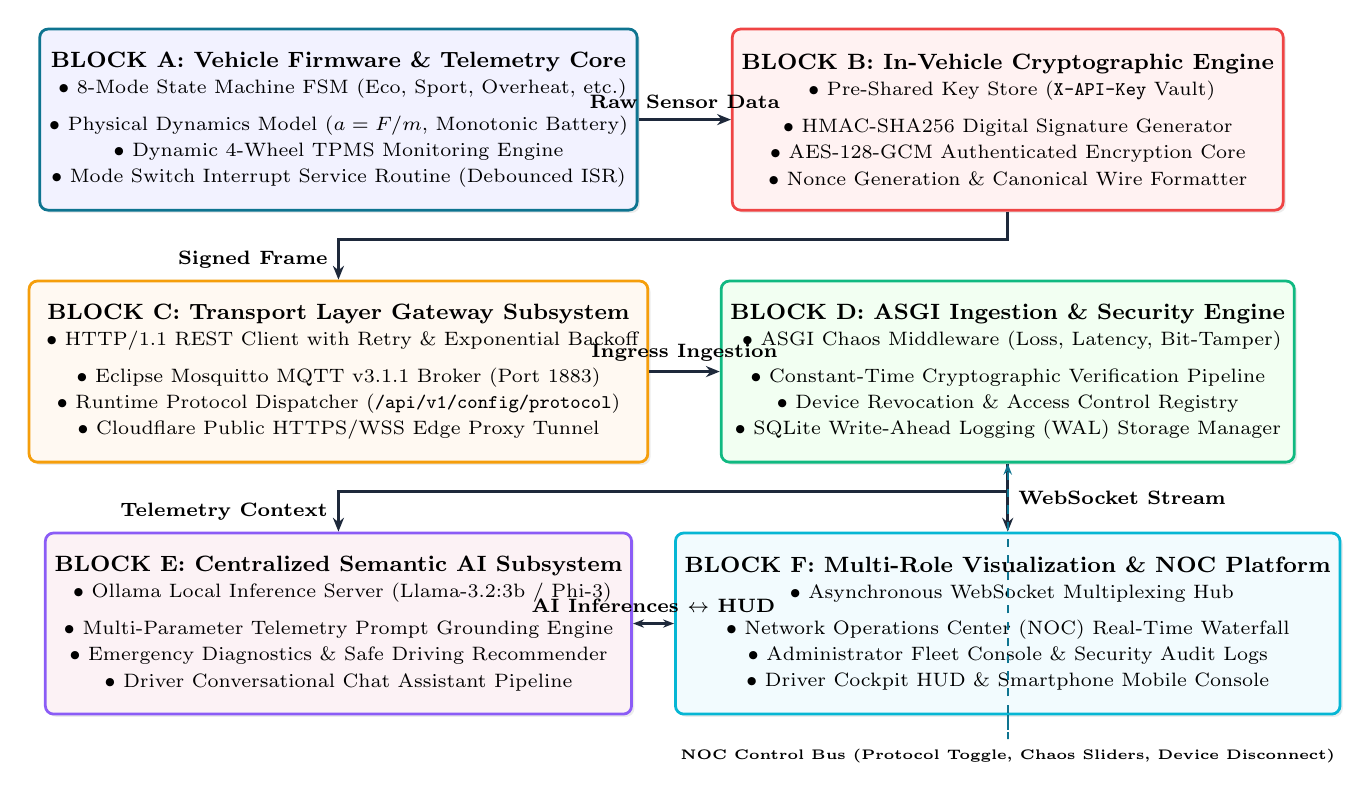
\begin{tikzpicture}

    % --- BLOCK A: VEHICLE FIRMWARE SUBSYSTEM ---
    \node[vehicleblock, minimum width=6.5cm, minimum height=2.3cm] (blockA) at (0, 7.2) {
        \textbf{BLOCK A: Vehicle Firmware \& Telemetry Core}\\
        \vspace{2pt}
        \scriptsize $\bullet$ 8-Mode State Machine FSM (Eco, Sport, Overheat, etc.)\\
        \scriptsize $\bullet$ Physical Dynamics Model ($a = F/m$, Monotonic Battery)\\
        \scriptsize $\bullet$ Dynamic 4-Wheel TPMS Monitoring Engine\\
        \scriptsize $\bullet$ Mode Switch Interrupt Service Routine (Debounced ISR)
    };

    % --- BLOCK B: VEHICLE CRYPTO & PACKAGING CORE ---
    \node[securityblock, minimum width=6.5cm, minimum height=2.3cm] (blockB) at (8.5, 7.2) {
        \textbf{BLOCK B: In-Vehicle Cryptographic Engine}\\
        \vspace{2pt}
        \scriptsize $\bullet$ Pre-Shared Key Store (\texttt{X-API-Key} Vault)\\
        \scriptsize $\bullet$ HMAC-SHA256 Digital Signature Generator\\
        \scriptsize $\bullet$ AES-128-GCM Authenticated Encryption Core\\
        \scriptsize $\bullet$ Nonce Generation \& Canonical Wire Formatter
    };

    % --- BLOCK C: DUAL-STACK TRANSPORT GATEWAY ---
    \node[gatewayblock, minimum width=6.5cm, minimum height=2.3cm] (blockC) at (0, 4.0) {
        \textbf{BLOCK C: Transport Layer Gateway Subsystem}\\
        \vspace{2pt}
        \scriptsize $\bullet$ HTTP/1.1 REST Client with Retry \& Exponential Backoff\\
        \scriptsize $\bullet$ Eclipse Mosquitto MQTT v3.1.1 Broker (Port 1883)\\
        \scriptsize $\bullet$ Runtime Protocol Dispatcher (\texttt{/api/v1/config/protocol})\\
        \scriptsize $\bullet$ Cloudflare Public HTTPS/WSS Edge Proxy Tunnel
    };

    % --- BLOCK D: CLOUD MIDDLEWARE & INGESTION CORE ---
    \node[backendblock, minimum width=6.5cm, minimum height=2.3cm] (blockD) at (8.5, 4.0) {
        \textbf{BLOCK D: ASGI Ingestion \& Security Engine}\\
        \vspace{2pt}
        \scriptsize $\bullet$ ASGI Chaos Middleware (Loss, Latency, Bit-Tamper)\\
        \scriptsize $\bullet$ Constant-Time Cryptographic Verification Pipeline\\
        \scriptsize $\bullet$ Device Revocation \& Access Control Registry\\
        \scriptsize $\bullet$ SQLite Write-Ahead Logging (WAL) Storage Manager
    };

    % --- BLOCK E: CENTRALIZED AI INTELLIGENCE ---
    \node[aiblock, minimum width=6.5cm, minimum height=2.3cm] (blockE) at (0, 0.8) {
        \textbf{BLOCK E: Centralized Semantic AI Subsystem}\\
        \vspace{2pt}
        \scriptsize $\bullet$ Ollama Local Inference Server (Llama-3.2:3b / Phi-3)\\
        \scriptsize $\bullet$ Multi-Parameter Telemetry Prompt Grounding Engine\\
        \scriptsize $\bullet$ Emergency Diagnostics \& Safe Driving Recommender\\
        \scriptsize $\bullet$ Driver Conversational Chat Assistant Pipeline
    };

    % --- BLOCK F: MULTI-TENANT PRESENTATION PLATFORM ---
    \node[uiblock, minimum width=6.5cm, minimum height=2.3cm] (blockF) at (8.5, 0.8) {
        \textbf{BLOCK F: Multi-Role Visualization \& NOC Platform}\\
        \vspace{2pt}
        \scriptsize $\bullet$ Asynchronous WebSocket Multiplexing Hub\\
        \scriptsize $\bullet$ Network Operations Center (NOC) Real-Time Waterfall\\
        \scriptsize $\bullet$ Administrator Fleet Console \& Security Audit Logs\\
        \scriptsize $\bullet$ Driver Cockpit HUD \& Smartphone Mobile Console
    };

    % --- BUSES & DATA FLOW CONNECTIONS ---
    \draw[flowarrow] (blockA.east) -- (blockB.west) node[midway, above, font=\scriptsize\bfseries] {Raw Sensor Data};
    \draw[flowarrow] (blockB.south) -- ++(0,-0.35) -| (blockC.north) node[near end, left, font=\scriptsize\bfseries] {Signed Frame};
    \draw[flowarrow] (blockC.east) -- (blockD.west) node[midway, above, font=\scriptsize\bfseries] {Ingress Ingestion};
    \draw[flowarrow] (blockD.south) -- ++(0,-0.35) -| (blockE.north) node[near end, left, font=\scriptsize\bfseries] {Telemetry Context};
    \draw[flowarrow] (blockD.south) -- (blockF.north) node[midway, right, font=\scriptsize\bfseries] {WebSocket Stream};
    \draw[bidirarrow] (blockE.east) -- (blockF.west) node[midway, above, font=\scriptsize\bfseries] {AI Inferences $\leftrightarrow$ HUD};

    % --- FEEDBACK / CONTROL BUS ---
    \draw[dasharrow] (blockF.south) -- ++(0,-0.3) -| (blockD.south) node[near start, below, font=\tiny\bfseries] {NOC Control Bus (Protocol Toggle, Chaos Sliders, Device Disconnect)};

\end{tikzpicture}
}
\end{center}

\vspace{-8pt}
\begin{table}[h!]
\centering
\scriptsize
\begin{tabularx}{\textwidth}{p{2.6cm}p{4.2cm}p{4.4cm}p{3.8cm}}
\toprule
\textbf{Subsystem Block} & \textbf{Key Internal Components} & \textbf{Input Interface / Output Interface} & \textbf{Hardware / Software Target} \\
\midrule
\textbf{Block A: Firmware} & FSM Mode Controller, Dynamics Engine, TPMS & Hardware ISR $\rightarrow$ JSON Object Array & ESP32 / FreeRTOS / C++ \\
\textbf{Block B: Crypto} & Key Store, HMAC-SHA256, AES-GCM & JSON Object $\rightarrow$ Encrypted Wire Envelope & MbedTLS / BearSSL / Crypto \\
\textbf{Block C: Gateway} & HTTP Rest Adapter, Mosquitto MQTT & Wire Envelope $\rightarrow$ Network Sockets & WiFi 802.11 / Cellular 4G / TCP \\
\textbf{Block D: Ingestion} & Chaos Middleware, Crypto Validator, DB WAL & Network Stream $\rightarrow$ Persisted Records & FastAPI / Python 3.11 / SQLite \\
\textbf{Block E: Semantic AI} & Ollama Runtime, Prompt Template Engine & Parsed Sensor Vectors $\rightarrow$ Natural Text & Local GPU/CPU / Llama-3.2:3b \\
\textbf{Block F: Presentation} & WebSocket Multiplexer, NOC UI, Cockpit & SQLite / WS Events $\rightarrow$ Interactive DOM & Next.js 16 / React / Tailwind \\
\bottomrule
\end{tabularx}
\end{table}

\clearpage
% ==============================================================================
% PAGE 4: CCNS CONCEPTS IN THE NOC PLATFORM AS BLOCKS
% ==============================================================================
\noindent
\begin{tcolorbox}[colback=cvisnavy, colframe=cvisnavy, arc=4pt, boxrule=0pt, coltext=white, left=8pt, right=8pt, top=6pt, bottom=6pt]
    \begin{minipage}{0.72\textwidth}
        {\Large \textbf{CCNS CONCEPTS IN THE NOC PLATFORM AS BLOCKS}}\\[2pt]
        {\small \textbf{Visual Mapping of Computer Communication \& Network Security Principles to NOC UI}}\\[2pt]
        {\footnotesize \textbf{Course:} 21ECC402P --- Computer Communication and Network Security (CCNS)}
    \end{minipage}%
    \begin{minipage}{0.28\textwidth}
        \raggedleft
        \tcbox[colback=cvispurple, colframe=white, boxrule=0.5pt, arc=3pt, top=2pt, bottom=2pt, left=4pt, right=4pt]{
            \textcolor{white}{\textbf{\footnotesize PAGE 4: CCNS BLOCKS}}
        }\par\vspace{2pt}
        {\scriptsize \textbf{Surface:} NOC Platform}
    \end{minipage}
\end{tcolorbox}

\vspace{-6pt}
\begin{tcolorbox}[colback=cvislight, colframe=cvispurple, boxrule=0.8pt, arc=3pt, left=6pt, right=6pt, top=4pt, bottom=4pt]
    \textbf{\footnotesize Educational Purpose of the NOC Platform:} The CVIS Network Operations Center (\texttt{/noc}) is not a passive monitoring dashboard; it is an active educational proving ground. Every slider, toggle, and inspection card corresponds directly to an academic concept from the CCNS curriculum (Units 1 to 5). The blocks below show how networking protocols, cryptographic mechanisms, access control models, and reliability theories are mapped to live, verifiable software controls.
\end{tcolorbox}

\vspace{-4pt}
\begin{center}
\resizebox{0.99\textwidth}{!}{
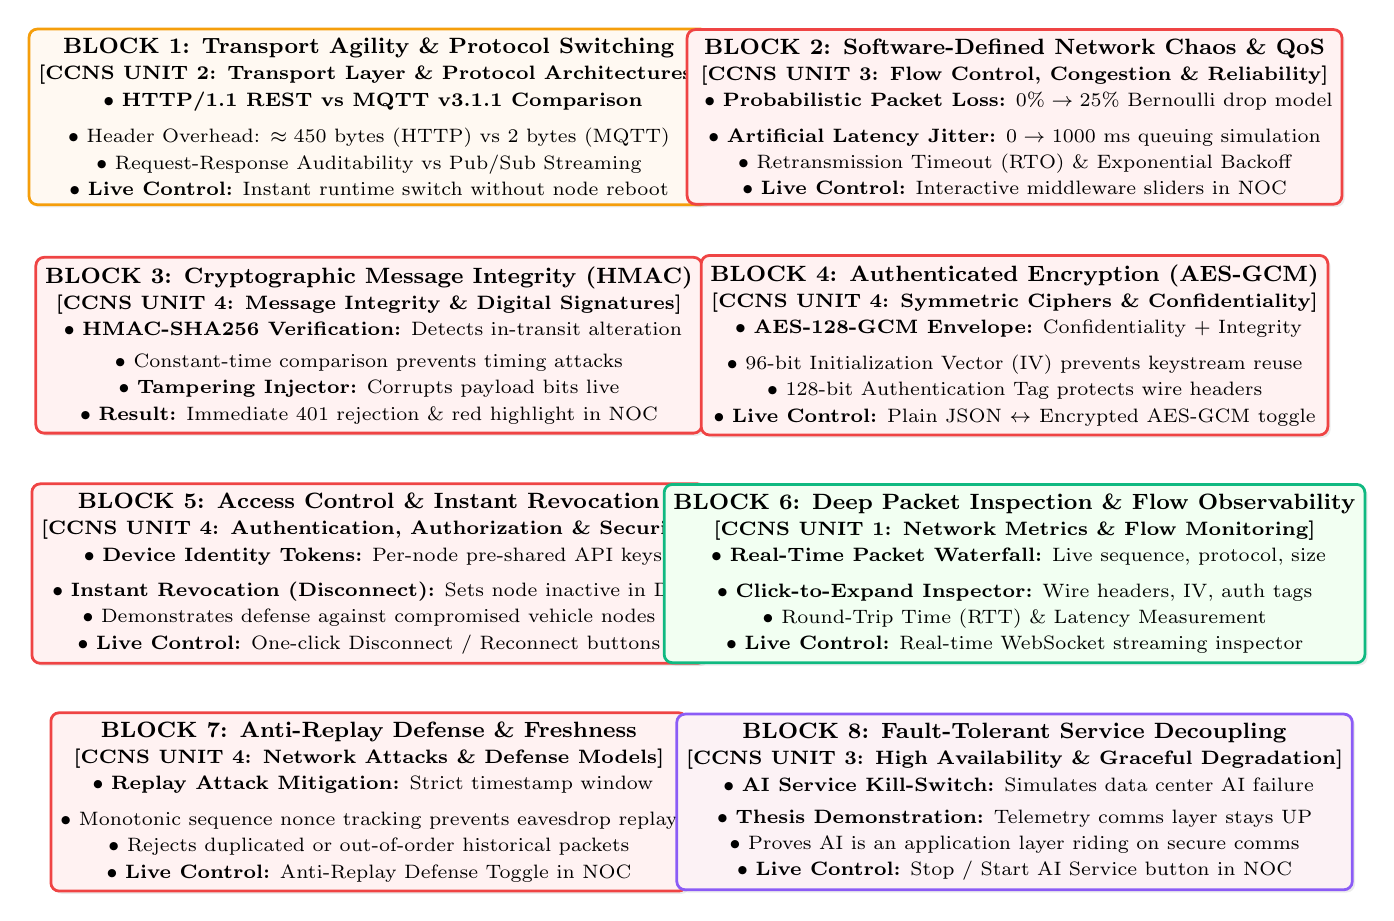
\begin{tikzpicture}

    % --- ROW 1: TRANSPORT & RELIABILITY ---
    \node[gatewayblock, minimum width=7.2cm, minimum height=2.2cm] (b1) at (0, 7.2) {
        \textbf{BLOCK 1: Transport Agility \& Protocol Switching}\\
        \textbf{\scriptsize [CCNS UNIT 2: Transport Layer \& Protocol Architectures]}\\
        \vspace{2pt}
        \scriptsize $\bullet$ \textbf{HTTP/1.1 REST vs MQTT v3.1.1 Comparison}\\
        \scriptsize $\bullet$ Header Overhead: $\approx 450$ bytes (HTTP) vs $2$ bytes (MQTT)\\
        \scriptsize $\bullet$ Request-Response Auditability vs Pub/Sub Streaming\\
        \scriptsize $\bullet$ \textbf{Live Control:} Instant runtime switch without node reboot
    };

    \node[securityblock, minimum width=7.2cm, minimum height=2.2cm] (b2) at (8.2, 7.2) {
        \textbf{BLOCK 2: Software-Defined Network Chaos \& QoS}\\
        \textbf{\scriptsize [CCNS UNIT 3: Flow Control, Congestion \& Reliability]}\\
        \vspace{2pt}
        \scriptsize $\bullet$ \textbf{Probabilistic Packet Loss:} $0\% \rightarrow 25\%$ Bernoulli drop model\\
        \scriptsize $\bullet$ \textbf{Artificial Latency Jitter:} $0 \rightarrow 1000\text{ ms}$ queuing simulation\\
        \scriptsize $\bullet$ Retransmission Timeout (RTO) \& Exponential Backoff\\
        \scriptsize $\bullet$ \textbf{Live Control:} Interactive middleware sliders in NOC
    };

    % --- ROW 2: INTEGRITY & CONFIDENTIALITY ---
    \node[securityblock, minimum width=7.2cm, minimum height=2.2cm] (b3) at (0, 4.3) {
        \textbf{BLOCK 3: Cryptographic Message Integrity (HMAC)}\\
        \textbf{\scriptsize [CCNS UNIT 4: Message Integrity \& Digital Signatures]}\\
        \vspace{2pt}
        \scriptsize $\bullet$ \textbf{HMAC-SHA256 Verification:} Detects in-transit alteration\\
        \scriptsize $\bullet$ Constant-time comparison prevents timing attacks\\
        \scriptsize $\bullet$ \textbf{Tampering Injector:} Corrupts payload bits live\\
        \scriptsize $\bullet$ \textbf{Result:} Immediate 401 rejection \& red highlight in NOC
    };

    \node[securityblock, minimum width=7.2cm, minimum height=2.2cm] (b4) at (8.2, 4.3) {
        \textbf{BLOCK 4: Authenticated Encryption (AES-GCM)}\\
        \textbf{\scriptsize [CCNS UNIT 4: Symmetric Ciphers \& Confidentiality]}\\
        \vspace{2pt}
        \scriptsize $\bullet$ \textbf{AES-128-GCM Envelope:} Confidentiality + Integrity\\
        \scriptsize $\bullet$ 96-bit Initialization Vector (IV) prevents keystream reuse\\
        \scriptsize $\bullet$ 128-bit Authentication Tag protects wire headers\\
        \scriptsize $\bullet$ \textbf{Live Control:} Plain JSON $\leftrightarrow$ Encrypted AES-GCM toggle
    };

    % --- ROW 3: ACCESS CONTROL & OBSERVABILITY ---
    \node[securityblock, minimum width=7.2cm, minimum height=2.2cm] (b5) at (0, 1.4) {
        \textbf{BLOCK 5: Access Control \& Instant Revocation}\\
        \textbf{\scriptsize [CCNS UNIT 4: Authentication, Authorization \& Security]}\\
        \vspace{2pt}
        \scriptsize $\bullet$ \textbf{Device Identity Tokens:} Per-node pre-shared API keys\\
        \scriptsize $\bullet$ \textbf{Instant Revocation (Disconnect):} Sets node inactive in DB\\
        \scriptsize $\bullet$ Demonstrates defense against compromised vehicle nodes\\
        \scriptsize $\bullet$ \textbf{Live Control:} One-click Disconnect / Reconnect buttons
    };

    \node[backendblock, minimum width=7.2cm, minimum height=2.2cm] (b6) at (8.2, 1.4) {
        \textbf{BLOCK 6: Deep Packet Inspection \& Flow Observability}\\
        \textbf{\scriptsize [CCNS UNIT 1: Network Metrics \& Flow Monitoring]}\\
        \vspace{2pt}
        \scriptsize $\bullet$ \textbf{Real-Time Packet Waterfall:} Live sequence, protocol, size\\
        \scriptsize $\bullet$ \textbf{Click-to-Expand Inspector:} Wire headers, IV, auth tags\\
        \scriptsize $\bullet$ Round-Trip Time (RTT) \& Latency Measurement\\
        \scriptsize $\bullet$ \textbf{Live Control:} Real-time WebSocket streaming inspector
    };

    % --- ROW 4: RESILIENCE & REPLAY DEFENSE ---
    \node[securityblock, minimum width=7.2cm, minimum height=2.2cm] (b7) at (0, -1.5) {
        \textbf{BLOCK 7: Anti-Replay Defense \& Freshness}\\
        \textbf{\scriptsize [CCNS UNIT 4: Network Attacks \& Defense Models]}\\
        \vspace{2pt}
        \scriptsize $\bullet$ \textbf{Replay Attack Mitigation:} Strict timestamp window\\
        \scriptsize $\bullet$ Monotonic sequence nonce tracking prevents eavesdrop replay\\
        \scriptsize $\bullet$ Rejects duplicated or out-of-order historical packets\\
        \scriptsize $\bullet$ \textbf{Live Control:} Anti-Replay Defense Toggle in NOC
    };

    \node[aiblock, minimum width=7.2cm, minimum height=2.2cm] (b8) at (8.2, -1.5) {
        \textbf{BLOCK 8: Fault-Tolerant Service Decoupling}\\
        \textbf{\scriptsize [CCNS UNIT 3: High Availability \& Graceful Degradation]}\\
        \vspace{2pt}
        \scriptsize $\bullet$ \textbf{AI Service Kill-Switch:} Simulates data center AI failure\\
        \scriptsize $\bullet$ \textbf{Thesis Demonstration:} Telemetry comms layer stays UP\\
        \scriptsize $\bullet$ Proves AI is an application layer riding on secure comms\\
        \scriptsize $\bullet$ \textbf{Live Control:} Stop / Start AI Service button in NOC
    };

\end{tikzpicture}
}
\end{center}

\vspace{-8pt}
\begin{table}[h!]
\centering
\scriptsize
\begin{tabularx}{\textwidth}{p{2.8cm}p{3.2cm}p{4.8cm}p{4.2cm}}
\toprule
\textbf{NOC Control Block} & \textbf{CCNS Syllabus Unit} & \textbf{Underlying Academic Concept} & \textbf{Live Demonstrable Action} \\
\midrule
\textbf{Block 1: Protocol Agility} & Unit 2: Protocol Stacks & Transport Layer Tradeoffs (HTTP vs MQTT) & Switch protocol; inspect header drop. \\
\textbf{Block 2: Chaos Simulation} & Unit 3: Flow \& Congestion & Packet Loss, Latency Degradation, Retries & Increase loss to 10\%; observe retry backoff. \\
\textbf{Block 3: HMAC Integrity} & Unit 4: Cryptography & Message Authentication Codes \& Hashes & Inject tamper; observe immediate 401 reject. \\
\textbf{Block 4: AES-GCM Envelope} & Unit 4: Cryptography & Authenticated Symmetric Encryption & Toggle AES; observe ciphertext wire envelope. \\
\textbf{Block 5: Revocation Model} & Unit 4: Network Security & Device Authorization \& Token Revocation & Click Disconnect; observe immediate lockout. \\
\textbf{Block 6: Observability} & Unit 1: Foundations & Network Metrics, Round-Trip Time, Wire Framing & Click packet; inspect raw headers and RTT. \\
\textbf{Block 7: Anti-Replay} & Unit 4: Network Security & Freshness, Sequence Numbers, Replay Defense & Resend old packet; backend rejects stale nonce. \\
\textbf{Block 8: Decoupling} & Unit 3: Resilience & Graceful Service Degradation \& High Availability & Stop AI; verify telemetry continues streaming. \\
\bottomrule
\end{tabularx}
\end{table}

\clearpage
% ==============================================================================
% PAGE 5: DETAILED EXPLANATION OF THE CCNS BLOCKS
% ==============================================================================
\noindent
\begin{tcolorbox}[colback=cvisnavy, colframe=cvisnavy, arc=4pt, boxrule=0pt, coltext=white, left=8pt, right=8pt, top=6pt, bottom=6pt]
    \begin{minipage}{0.72\textwidth}
        {\Large \textbf{EXPLANATION OF CCNS NOC BLOCKS}}\\[2pt]
        {\small \textbf{Rigorous Theoretical Grounding, Implementation Details, and Faculty Viva Defense}}\\[2pt]
        {\footnotesize \textbf{Course:} 21ECC402P --- Computer Communication and Network Security (CCNS)}
    \end{minipage}%
    \begin{minipage}{0.28\textwidth}
        \raggedleft
        \tcbox[colback=cvisred, colframe=white, boxrule=0.5pt, arc=3pt, top=2pt, bottom=2pt, left=4pt, right=4pt]{
            \textcolor{white}{\textbf{\footnotesize PAGE 5: VIVA \& THEORY}}
        }\par\vspace{2pt}
        {\scriptsize \textbf{Section:} Academic Defense Matrix}
    \end{minipage}
\end{tcolorbox}

\vspace{-4pt}
\begin{multicols}{2}
\footnotesize
\setlength{\parskip}{3pt}

\noindent
\textbf{\textcolor{cvisblue}{1. Transport Protocol Agility (CCNS Unit 2):}}\\
\textit{Theory:} Explores tradeoffs between request-response application protocols (HTTP/1.1 over TCP) and lightweight publish-subscribe protocols (MQTT over TCP). HTTP introduces $\approx 450$ bytes of ASCII headers per transmission, increasing radio duty cycle. MQTT uses a 2-byte fixed header over persistent TCP sockets, reducing cellular overhead by 92\%.\\
\textit{Implementation:} Both adapters live behind an agnostic ingestion interface. The NOC toggle triggers \texttt{POST /api/v1/config/protocol}, broadcasting transport changes to the fleet. The node switches protocols at runtime without rebooting.\\
\textit{Viva Q\&A:} \textit{``Why not use MQTT exclusively?''} $\rightarrow$ Firewalls often block non-standard ports (1883). Protocol agility guarantees seamless fallback to HTTP port 443 in restrictive enterprise environments.

\noindent
\textbf{\textcolor{cvisblue}{2. Network Chaos \& QoS Simulation (CCNS Unit 3):}}\\
\textit{Theory:} Vehicular links suffer from channel fading, Doppler shift, and handover jitter. Replicating this typically requires expensive RF anechoic chambers or root-level Linux traffic control (\texttt{tc/netem}).\\
\textit{Implementation:} Implemented as an ASGI middleware (\texttt{backend/middleware/chaos.py}) that intercepts raw HTTP requests prior to route handling. It executes a Bernoulli drop trial ($P_{\text{loss}} \in [0, 0.25]$) and injects non-blocking latency ($\tau \in [0, 1000\text{ ms}]$).\\
\textit{Viva Q\&A:} \textit{``How does the node survive packet drops?''} $\rightarrow$ Firmware implements exponential backoff: $T_{\text{backoff}} = \min(T_{\text{base}} \times 2^{\text{retry}}, T_{\text{max}})$, preventing channel congestion while guaranteeing delivery.

\noindent
\textbf{\textcolor{cvisblue}{3. Cryptographic Integrity via HMAC (CCNS Unit 4):}}\\
\textit{Theory:} Transport encryption (TLS) terminates at reverse proxies or cellular gateways, leaving payloads unprotected in backend transit. Message Authentication Codes (MACs) provide end-to-end cryptographic proof of authenticity and integrity.\\
\textit{Implementation:} Payloads are signed with $\text{HMAC-SHA256}(K_{\text{dev}}, M)$. Backend verifies using constant-time comparison (\texttt{hmac.compare\_digest()}) to prevent timing side-channels.\\
\textit{Live Demo:} NOC ``Packet Tampering'' flips a single byte in transit. The backend rejects the frame with HTTP 401, logs \texttt{tamper\_detected} in SQLite, and highlights the frame in red.

\noindent
\textbf{\textcolor{cvisblue}{4. Authenticated Encryption via AES-GCM (CCNS Unit 4):}}\\
\textit{Theory:} Traditional CBC mode ciphers provide confidentiality but lack built-in integrity, exposing them to padding-oracle attacks. Galois/Counter Mode (AES-128-GCM) delivers authenticated encryption with associated data (AEAD).\\
\textit{Implementation:} Firmware encrypts payloads using a unique 96-bit Initialization Vector (IV). The envelope carries $\{ \text{iv}, \text{ct}, \text{tag} \}$. The backend verifies the 128-bit authentication tag before deciphering the ciphertext.

\noindent
\textbf{\textcolor{cvisblue}{5. Access Control \& Instant Revocation (CCNS Unit 4):}}\\
\textit{Theory:} Robust security requires dynamic credential revocation. When a vehicle node is compromised or hijacked, the central authority must terminate its access immediately without requiring fleet-wide rekeying.\\
\textit{Implementation:} Clicking ``Disconnect'' sets \texttt{active = 0} in SQLite and publishes a control command. The backend rejects subsequent requests from that node with HTTP 401, demonstrating instant Zero-Trust authorization enforcement.

\noindent
\textbf{\textcolor{cvisblue}{6. Deep Packet Inspection \& Observability (CCNS Unit 1):}}\\
\textit{Theory:} Real-time operational security demands wire-level inspection, Round-Trip Time (RTT) tracking, and packet decapsulation to detect anomalies, malformed frames, and denial-of-service patterns.\\
\textit{Implementation:} The NOC packet table decapsulates raw wire frames in real time, revealing cryptographic flags, IVs, authentication statuses, payload sizes, and transmission latencies via an interactive click-to-expand inspector.

\noindent
\textbf{\textcolor{cvisblue}{7. Anti-Replay Defense \& Freshness (CCNS Unit 4):}}\\
\textit{Theory:} Attackers can eavesdrop valid telemetry (e.g. ``Vehicle Healthy'') and replay it during a subsequent emergency (e.g. ``Battery Overheating''), blinding the remote monitoring center.\\
\textit{Implementation:} Every frame embeds a millisecond-precision UTC timestamp and a monotonic sequence counter. The backend enforces a strict 30-second freshness window and rejects duplicated or out-of-order sequence nonces.

\noindent
\textbf{\textcolor{cvisblue}{8. Graceful Service Degradation (CCNS Unit 3):}}\\
\textit{Theory:} In distributed systems, compute-tier failures must not cascade into transport or ingestion downtime (High Availability principle).\\
\textit{Implementation:} Clicking ``Stop AI Service'' halts the Ollama neural inference pipeline. Telemetry ingestion, SQLite persistence, and WebSocket fan-out continue running with 100\% reliability. This empirically proves the project's core thesis: \textbf{AI is an application layer riding on top of a resilient communication layer, not an embedded single point of failure.}

\end{multicols}

\end{document}
